% !TeX root = report_example.tex
\newcommand*{\MyHeaderPath}{.}% This path definition is also passed to inside the header files.
\newcommand*{\PathToAssets}{../assets}%
\newcommand*{\PathToOutput}{../output}%
\newcommand*{\PathToBibFile}{bibliography.bib}%


%%%%%%%%%%%%%%%%%%%%%%%%%%%%%%%%%%%%%%
%% This file is compiled with XeLaTex.
%%%%%%%%%%%%%%%%%%%%%%%%%%%%%%%%%%%%%%

\documentclass[12pt]{article}
%\documentclass[reqno]{amsart}
%\documentclass[titlepage]{amsart}

%% {{{{
%% This package is already loaded by beamer
% https://tex.stackexchange.com/questions/314344/beamer-presentation-compile-error
\usepackage{graphicx}
%% }}}}

%http://tex.stackexchange.com/questions/36797/how-can-i-make-todonotes-use-all-of-the-margin
\usepackage{fullpage}
%\usepackage{showframe}
% \usepackage[paperwidth=210mm,
%             paperheight=297mm,
%             left=50pt,
%             top=50pt,
%             textwidth=345pt,
%             marginparsep=25pt,
%             marginparwidth=150pt,
%             textheight=692pt,
%             footskip=50pt]
%            {geometry}

%% {{{{
% https://tex.stackexchange.com/questions/9796/how-to-add-todo-notes
\usepackage{xargs} % Use more than one optional parameter in a new commands 
\usepackage[dvipsnames]{xcolor}
% \newcommandx{\todoproposal}[2][1=]{\todo[linecolor=Plum,backgroundcolor=Plum!25,bordercolor=Plum,#1]{#2}}
\newcommandx{\todoproposal}[2][1=]{\todo[disable, linecolor=Plum,backgroundcolor=Plum!25,bordercolor=Plum,#1]{#2}}
% \newcommandx{\tododraft}[2][1=]{\todo[#1]{#2}}
\newcommandx{\tododraft}[2][1=]{\todo[disable, #1]{#2}}
% \newcommandx{\thiswillnotshow}[2][1=]{\todo[disable,#1]{#2}}
%% Math environment in todo note
%
% https://tex.stackexchange.com/questions/298404/todonotes-and-reserveda-nested-itemize-enumerate-environments/298405#298405
\newcommand\todoin[2][]{\todo[inline, caption={2do}, #1]{
\begin{minipage}{\textwidth-4pt}#2\end{minipage}}}
% \newcommand\todoin[2][]{\todo[disable, inline, caption={2do}, #1]{
% \begin{minipage}{\textwidth-4pt}#2\end{minipage}}}
%% }}}}


%% {{{{
%http://tex.stackexchange.com/questions/44858/adding-the-word-appendix-to-table-of-contents-in-latex
\usepackage[titletoc, page]{appendix}
%% }}}}

%% {{{{
	
%I'm using this package to put todo notes into my document. Then, I can
%use it to put a list of the todo notes at the end of the document.
\usepackage[textsize=footnotesize]{todonotes}
% \usepackage[disable=true, colorinlistoftodos,prependcaption,textsize=footnotesize]{todonotes}
%This package has some conficts with amsart. To resolve this, I use
%the following code.
\makeatletter
\providecommand\@dotsep{5}
\def\listtodoname{List of Todos}
\def\listoftodos{\@starttoc{tdo}\listtodoname}
\makeatother
%I got this workaround code from the package's documentation:
%http://get-software.net/macros/latex/contrib/todonotes/todonotes.pdf

% %\newcounter{chapter}
% %\numberwithin{section}{chapter}
% \theoremstyle{mydefinition}
% \newtheorem{exercise}{Exercise}
% \newcommand{\newproblem}[2]{\setcounter{exercise}{#1}\addtocounter{exercise}{
% -1}\begin{exercise}#2\end{exercise}}
% \newcommand{\setcontext}[2]{\setcounter{chapter}{#1}\setcounter{section}{#2}}

% \newtheorem*{remark}{Remark}

%% }}}}


%% {{{{
% Bibliography as numbered section
% https://tex.stackexchange.com/questions/88890/how-to-get-the-references-section-to-be-numbered-as-if-it-were-created-via-sect
\usepackage[numbib]{tocbibind}
%% }}}}


%%%%%%%%%%%%5
%%%% >>>>

%%%%%%%%%%%%5


%%%%%%%%%%%%%%%%%%%%%%%%
%% Section Styling
%%%%%%%%%%%%%%%%%%%%%%%%%

 \usepackage{titlesec}

% %\titleformat*{\subsection}{\newpage \Large \bfseries}
% \titleformat*{\subsubsection}{\large\itshape}

% \usepackage[explicit]{titlesec}

% %Start section with new page
% %http://tex.stackexchange.com/questions/9497/start-new-page-with-each-section
% \newcommand{\sectionbreak}{\clearpage}

% %Underlining ruler for subsections
% %http://tex.stackexchange.com/questions/84061/how-can-i-make-a-bold-horizontal-rule-under-each-section-title
% \titleformat{\section}
%   {\normalfont\LARGE\bfseries}
%   {
%   \thesection
%   }
%   {1em}
%   {#1}
%   [{\titlerule[0.8pt]}]

% \titleformat{\subsection}
%   {\normalfont\Large\bfseries}
%   {\thesubsection}
%   {1em}
%   {#1}

% \titleformat{\subsubsection}
%   {\normalfont\normalsize\itshape}
%   {\thesubsubsection}
%   {1em}
%   {#1}


% Change format of \paragraph{...}
% http://tex.stackexchange.com/questions/3881/formatting-a-paragraph-to-look-like-a-section
% \titleformat{\paragraph}[hang]{\normalfont\normalsize\itshape}{\theparagraph}{1em}{}
% \titlespacing*{\paragraph}{0pt}{3.25ex plus 1ex minus .2ex}{1em}


%%%%%%%%%%%%%%%%%%%%%%%%%%%%%%%%%%%%%%%%%%%%%%
%% Change section styling for HW documents %%
%%%%%%%%%%%%%%%%%%%%%%%%%%%%%%%%%%%%%%%%%%%%%%

%%%
% This first method uses the base LaTeX package:
% http://tex.stackexchange.com/questions/85011/section-and-subsection-heading-style

%\def\@seccntformat#1{\csname the#1\endcsname\quad} %default

%\def\@seccntformat#1{Problem \csname the#1\endcsname\quad} 

% %%% 
% % This next one uses the `titlesec` packages. The references I used are
% % here:
% % http://tex.stackexchange.com/questions/140447/changing-section-heading-style
% % http://tex.stackexchange.com/questions/37189/number-subsections-and-subsubsections-but-not-sections
% \usepackage{bookmark}
% \usepackage{titlesec}
% \titleformat{\section}
%   {\normalfont\bfseries\Large}{Problem \thesection}{1em}{}
% \titleformat{\subsection}
%   {\normalfont\large\itshape}{\thesubsection}{1em}{}
% \titleformat{\subsubsection}
%   {\normalfont\normalsize\itshape}{\thesubsubsection}{1em}{}

% % Add proper labels to PDF bookmarks.
% % http://tex.stackexchange.com/questions/156530/how-to-change-the-pdfbookmark-titles-hyperref
% \makeatletter
% \bookmarksetup{%
%   addtohook={%
%     \ifnum\toclevel@section=\bookmarkget{level}\relax
%       \renewcommand*{\numberline}[1]{Problem #1 }%
%     \fi
%   },
% }



%Option to number subsection with letters
% http://tex.stackexchange.com/questions/74529/sections-indexed-with-numbers-subsections-with-letters
% \renewcommand{\thesection}{\Alph{section}}
% \renewcommand{\thesubsubsection}{\thesubsection.\alph{subsubsection}}
% %%%%%%%%%%%%%%%%%%%%%%%%%%%%%%%%%%%%%%%%%%%%%

%% {{{{
%Links, esp. from table of contents
% http://timmurphy.org/2014/03/11/latex-table-of-contents-with-clickable-links/
\usepackage{hyperref}
\hypersetup{
    colorlinks=true, % make the links colored
    linkcolor=blue, % color TOC links in blue
    urlcolor=red, % color URLs in red
    linktoc=all, % 'all' will create links for everything in the TOC
    %citecolor=gray
    citecolor=blue
    }
%% }}}}

\usepackage{setspace}
%% Deal with warnings

% -- Temporarily filter warning. "remreset package is obsolete". This package is likely innocuous.
% https://tex.stackexchange.com/questions/438543/what-to-do-when-an-actively-maintained-package-requires-an-obsolete-package
\RequirePackage{silence}
\WarningFilter{remreset}{The remreset package}

% -- Todo notes margin warning:
\setlength {\marginparwidth }{2cm}

%https://tex.stackexchange.com/questions/3473/blackboard-bold-variants-for-greek-letters
\usepackage[bbgreekl]{mathbbol}

\usepackage{amsmath, amsfonts, amscd, amssymb, amsthm}
\usepackage{url}
\usepackage{enumerate}
\usepackage{float}
\usepackage{bbm}
\usepackage{color,soul}
\usepackage{thmtools}
\usepackage{threeparttable}
\usepackage[bottom]{footmisc}
\usepackage{rotating}

%% {{{{

%% When Caption is too wide:
% https://tex.stackexchange.com/questions/110393/too-wide-figure-caption/110453
% \captionsetup{width=0.8\textwidth}

% \usepackage[skip=4pt,font=footnotesize, width=\textwidth]{caption}
\usepackage[font=small]{caption}
% \usepackage{caption}
\usepackage{subcaption}
%% }}}}

%% {{{{
%% Bibliography
\usepackage[round,sort,comma,authoryear]{natbib}
% Include in main .tex file: \newcommand*{\MyHeaderPath}{..path_to_header_files..}%
% \bibliographystyle{rusnat}
% \bibliographystyle{plainnat}   % this means that the order of references
%% }}}}


\usepackage[export]{adjustbox}

%% Biblatex
% \usepackage[natbib=true]{biblatex}
% \addbibresource{../../My_Collection.bib}


\usepackage{mathtools}


%% {{{{
% Scalable font and better handling of accents, etc.
% https://tex.stackexchange.com/questions/664/why-should-i-use-usepackaget1fontenc
% https://tex.stackexchange.com/a/10708/41208
% \usepackage[T1]{fontenc}
\usepackage{lmodern}
%% }}}}

%% {{{
% Doesn't work with beamer
% https://tex.stackexchange.com/questions/314344/beamer-presentation-compile-error#comment766741_314344
% Anyway, loading the packages in different order solves the issue: load bm last. I suggest the order inputenc, fontenc, babel if needed, lmodern, mathtools and finally bm
\usepackage{bm}
%% }}}



\usepackage{dcolumn}

%% Force LaTeX image to appear in the section in which it's declared [duplicate]
% https://tex.stackexchange.com/questions/32598/force-latex-image-to-appear-in-the-section-in-which-its-declared
\usepackage[section]{placeins}

%% Used for making landscape (sidewaystable) tables
%
% From here: https://latex.org/forum/viewtopic.php?t=1493
% Creates sideways table environment 
\usepackage{rotating}


%% For use in making tables with multiple panels
%
% See here: https://tex.stackexchange.com/questions/27971/tables-with-multiple-panels-in-latex-r-and-sweave
\usepackage{tabularx}% http://ctan.org/pkg/tabularx
\newcolumntype{Y}{>{\raggedleft\arraybackslash}X}% raggedleft column X

%% For use in raggedright text justification in regular tabular tables
%
% See here: https://tex.stackexchange.com/questions/12703/how-to-create-fixed-width-table-columns-with-text-raggedright-centered-raggedlef
\usepackage{array}
\newcolumntype{L}[1]{>{\raggedright\let\newline\\\arraybackslash\hspace{0pt}}m{#1}}
\newcolumntype{C}[1]{>{\centering\let\newline\\\arraybackslash\hspace{0pt}}m{#1}}
\newcolumntype{R}[1]{>{\raggedleft\let\newline\\\arraybackslash\hspace{0pt}}m{#1}}

% How to add a forced line break inside a table cell
% https://tex.stackexchange.com/questions/2441/how-to-add-a-forced-line-break-inside-a-table-cell
\usepackage{pbox}


%% For use in making landscape tables
% https://tex.stackexchange.com/questions/3930/how-to-rotate-landscape-table-page-in-pdf
% An interesting alternative that also works is https://tex.stackexchange.com/questions/37220/how-to-adjust-or-remove-page-numbers-on-a-landscape-page-within-a-portrait-docum
\usepackage{geometry}
\usepackage{pdflscape}


\usepackage{bibentry}
\makeatletter
%http://tex.stackexchange.com/questions/141446/problem-of-duplicate-identifier-when-using-bibentry-and-hyperref
\renewcommand\bibentry[1]{\nocite{#1}{\frenchspacing
\@nameuse{BR@r@#1\@extra@b@citeb}}}
\makeatother


% %%%% <<<<

% %% Professional Looking Code listings
% %% http://stackoverflow.com/questions/741985/latex-source-code-listing-like-in-professional-books

% %\usepackage{color}
% \usepackage{xcolor}
% \usepackage{listings}

% %\usepackage{caption}
% \DeclareCaptionFont{white}{\color{white}}
% \DeclareCaptionFormat{listing}{\colorbox{gray}{\parbox{\textwidth}{#1#2#3}}}
% \captionsetup[lstlisting]{format=listing,labelfont=white,textfont=white}

% %% Alternative Font for Code Listings
% %% http://tex.stackexchange.com/questions/33685/set-the-font-family-for-lstlisting
% \usepackage{courier}

% \lstset{basicstyle=\footnotesize\ttfamily,breaklines=true}
% \lstset{framextopmargin=50pt,frame=bottomline}

% %% Line Numbers
% \lstset
% { %Formatting for code in appendix
%     %language=Matlab,
%     numbers=left,
%     stepnumber=1,
%     showstringspaces=false,
%     tabsize=1,
%     breaklines=true,
%     breakatwhitespace=false,
% }

% %% Line Numbers starting form an arbitrary number
% %% http://tex.stackexchange.com/questions/61030/how-can-i-start-the-line-numbering-of-my-listing-by-an-arbitrary-number

% % \begin{lstlisting}[firstnumber=100]
% % for i:=maxint to 0 do
% % begin
% % { do nothing }
% % end;
% % \end{lstlisting}

% %%%% >>>>

%%%% <<<<

%% Examples of using underset and underbrace

% $$
% \frac{\dd \pi^2}{\dd K_1} = 
%   \underbrace{\pd{\pi^2}{K_1} }_\text{direct effect}
%   + 
%   \underbrace{\pd{\pi^2}{x_1^*} \pd{x_1^*}{K_1}}_\text{strategic effect}
%   + \underset{\text{due to the envelope theorem}}
%   {\cancel{ \pd{\pi^2}{x_2^*}\pd{x_2^*}{K_1}}}
% $$
%%%% >>>>


%% Aligning numbers by decimal points in table columns
%https://tex.stackexchange.com/questions/2746/aligning-numbers-by-decimal-points-in-table-columns
\usepackage{siunitx}
% From here:https://ctan.org/pkg/siunitx
% Don't intepret comma as decimal marker
\sisetup{
input-decimal-markers = .
}



%%%% <<<<
%% Packages for tables
\usepackage{booktabs}
\usepackage{multirow}
%\usepackage[table,xcdraw]{xcolor}
%I got the following one from here: http://stackoverflow.com/questions/790932/how-to-wrap-text-in-latex-tables
\usepackage{tabulary}
%% Example Table
% \begin{figure}[h!]
% \centering
% \begin{tabulary}{\linewidth}{C|C|C}
% \toprule
% Actions & Inflow at time $t$ & Inflow at time $t + \dd t$     \\ \midrule
% Buy and sell call & $-C$ & $C + \dd C$ \\ \hline
% Short $\alpha$ shares & $\alpha S$ & $-\alpha (S + \dd S)$ \\ \hline
% Buy and sell $\beta$ of option $\hat C$ & $-\beta \hat C$ & $\beta (\hat C + \dd \hat C)$ \\ \hline
% Borrow & $C - \alpha S + \beta \hat C$ & $-(1+r)(C - \alpha S + \beta \hat C)$ \\ \hline
% Net & 0 & $C + \dd C - \alpha (S + \dd S) + \beta (\hat C + \dd \hat C)
%  - (1+r) (C - \alpha S + \beta \hat C)$
% \\ \hline
% \bottomrule
% \end{tabulary} 
% \end{figure}

%itemize in table:
%  http://tex.stackexchange.com/questions/150492/how-to-use-itemize-in-table-environment
\newcommand{\tabitem}{~~\llap{\textbullet}~~}

%useful for spacining:
% http://tex.stackexchange.com/questions/267601/invisible-and-unselectable-text
%%%% >>>>

%%%% <<<<<<
%% Text Box:
% http://tex.stackexchange.com/questions/36524/how-to-put-a-framed-box-around-text-math-enviroment
\usepackage{tcolorbox}
%% Example:

% \begin{tcolorbox}
% blablabla
% \begin{align}
% E &= mc^2 & \text{Formula of the universe}
% \end{align}
% Hoaray
% \end{tcolorbox}

%% http://tex.stackexchange.com/questions/172475/how-can-i-define-a-custom-tcolorbox-environment-with-color-as-a-parameter

% new tcolorbox environment
% #1: tcolorbox options
% #2: color
% #3: box title
\newtcolorbox{textbox}[3][]
{
colframe = #2!25,
colback  = #2!10,
coltitle = #2!20!black,  
title    = #3,
#1,
}
%%%% >>>>>>

%%%% <<<<<<
%%%%%%%%%%%%%%%%%%%%%%%%
%% Cancel out math terms
%http://tex.stackexchange.com/questions/75525/how-to-write-crossed-out-math-in-latex
\usepackage[makeroom]{cancel}
%% Examples:
%%
% \verb|\cancel{5y}|:
% \[ x+\cancel{5y}=0\]
% \verb|\bcancel{5y}|:
% \[ x+\bcancel{5y}=0\]
% \verb|\xcancel{5y}|:
% \[ x+\xcancel{5y}=0\]
% \verb|\cancelto{\infty}{5y}|:
% \[ x+\cancelto{\infty}{5y}=0\]

% The first three commands work in text mode also i.e., \cancel{5y}, \bcancel{5y} and 
% \xcancel{5y} works but \verb|\cancelto{\infty}{5y}| is not. 
%%%% >>>>>>

\usepackage{lscape}
%\begin{landscape}
%...
%\end{landscape}

%I'm using this for the \intertext and \shortintertex commands
%to be used with the align environment from amsmath
\usepackage{mathtools}


%%%%%%%%%%%%%%%%
%Custom commands
%%%%%%%%%%%%%%%%


%%%%%%%%%%%%%%%%%%%%%%%%%%%%%%%%%%%%%%%%%%%%%%%%%%%%%
%%Custom commands for common mathematical expressions



%QED "grave" symbol
\renewcommand{\qed}{\begin{flushright} $\square$ \end{flushright}}
%vector of ones
\newcommand{\1}{\mathbbm{1}}
\newcommand{\E}{\mathbbm{E}}
%differential d
\newcommand{\dd}{\, \mathrm{d}}
%variance and covariance
\newcommand{\Var}{\text{Var}}
\newcommand{\Std}{\text{Std}}
\newcommand{\Cov}{\text{Cov}}
\newcommand{\Corr}{\text{Corr}}
\newcommand{\pd}[2]{\frac{\partial #1}{\partial #2}}
\renewcommand{\t}{\prime}


%% Underline, underbar, ubar, munderbar
% http://tex.stackexchange.com/questions/163280/underbar-changing-the-style-of-font-but-bar-not-why
\usepackage{accents}
\newcommand{\ubar}[1]{\underaccent{\bar}{#1}}

%% Rename hats and tildes
\let\smallhat\hat
\renewcommand{\hat}{\widehat}
\let\smalltilde\tilde
\renewcommand{\tilde}{\widetilde}

% https://tex.stackexchange.com/questions/43335/how-to-write-is-distributed-as-under-a-certain-hypothesis
%% iid over \sim
\makeatletter
\newcommand{\distas}[1]{\mathbin{\overset{#1}{\kern\z@\sim}}}%
\newsavebox{\mybox}\newsavebox{\mysim}
\newcommand{\distras}[1]{%
  \savebox{\mybox}{\hbox{\kern3pt$\scriptstyle#1$\kern3pt}}%
  \savebox{\mysim}{\hbox{$\sim$}}%
  \mathbin{\overset{#1}{\kern\z@\resizebox{\wd\mybox}{\ht\mysim}{$\sim$}}}%
  }

%% Deemphasizing Text {{{
% https://latex.org/forum/viewtopic.php?t=17731
\newcommand{\light}[1]{{\footnotesize \textcolor{gray}{#1}}}
% \light{This is grayed-out}  
% }}}

%%%%%%%%%%%%%%%%%%%%%%%%%%%%%%%
%%Document Specific Commands%%%
%%%%%%%%%%%%%%%%%%%%%%%%%%%%%%%%


%%%%% {{{{
% Theroems

% \newcommand{\bm}[1]{\begin{bmatrix}#1 \end{bmatrix}}
\newtheorem{goal}{Project Goal}

% https://en.wikibooks.org/wiki/LaTeX/Theorems#Theorem_counters
%\newtheorem{proposition}{Proposition}
\newtheorem{proposition}{Proposition}
\newtheorem{mylemma}[proposition]{Lemma}
\newtheorem{mycorollary}[proposition]{Corollary} 
\newtheorem{myassumption}[proposition]{Assumption} 
% OLD: Use proposition counter as `parent` %This comes from https://tex.stackexchange.com/a/381593/41208
% \newtheorem{theorem}{Theorem}[section]

\theoremstyle{definition}
\newtheorem{myexample}{Example}[section]
\theoremstyle{definition}
\newtheorem{mydefinition}[proposition]{Definition}


\newcommand\xqed[1]{%
  \leavevmode\unskip\penalty9999 \hbox{}\nobreak\hfill
  \quad\hbox{#1}}
\newcommand\demo{\xqed{$\triangle$}}

%%%%% }}}}


%% Needed for underbraces under matrix
\newlength{\bracewidth}
\newcommand{\myunderbrace}[2]{\settowidth{\bracewidth}{$#1$}#1\hspace*{-1\bracewidth}\smash{\underbrace{\makebox{\phantom{$#1$}}}_{#2}}}


%% Another method for braces under a matrix. This comes from
% https://tex.stackexchange.com/a/102468/41208
\newcommand\undermat[2]{%
  \makebox[0pt][l]{$\smash{\underbrace{\phantom{%
    \begin{matrix}#2\end{matrix}}}_{\text{$#1$}}}$}#2}



%%%% <<<<
%%%%%%%%%%%%%
%%Custom commands for quickly entering pictures

%Fast Picture
%Arguments {File}{ShortCaption}{LongCaption}{Label}
\newcommand{\fastpic}[4]{
\begin{figure}[H]
\centering
\includegraphics[width=3in]{#1}
\caption[#2]
{#3}
\label{#4}
\end{figure}
}

%A bigger picture
\newcommand{\bfastpic}[4]{
\begin{figure}[H]
\centering
\includegraphics[width=5in]{#1}
\caption[#2]
{#3}
\label{#4}
\end{figure}
}

%fast side-by-side picture
% Arguments--
% #1: filename
% #2: subcaption
% #3: subtag
% #4: filename
% #5: subcaption
% #6: subtag
% #7: supercaption
% #8: supertag
\newcommand{\fastpicTwo}[8]{
\begin{figure}[H]
\centering
\begin{subfigure}[b]{0.45\textwidth}
\includegraphics[width=\textwidth]{#1}
\caption{#2}
\label{#3}
\end{subfigure}
    ~ %add desired spacing between images, e. g. ~, \quad, \qquad, \hfill etc. 
      %(or a blank line to force the subfigure onto a new line)
      \begin{subfigure}[b]{0.45\textwidth}
      \includegraphics[width=\textwidth]{#4}
      \caption{#5}
      \label{#6}
      \end{subfigure}
      \caption{#7}\label{#8}
      \end{figure}

      }





\makeatother
%%%%%%%%%%%%%%%%%%%%%%%%%%%%%%%%%%%%%%%%%%%%%%%%%%%%%%%%%%%%%%%%%%%%%%%%%%
%%%%%%%%%%%%%%%%%%%%%%%%%%%%%%%%%%%%%%%%%%%%%%%%%%%%%%%%%%%%%%%%%%%%%%%%%%









\begin{document}
\title{
The Puzzle of Filtering Index Options
\\{\color{blue} \large UChicago WI 23: FINN 329\footnote{Taught by Jeremy Bejarano, jbejarano@uchicago.edu }}
}
% {\color{blue} \large Preliminary. Do not distribute.}
% }

\author{
Viren Desai, Harrison Holt, Ian Hammock 
  % \newline 
  % \hspace{3pt} \indent \hspace{3pt}
  % % I am immensely grateful to...
}
% \maketitle
\begin{titlepage}
% \input{cover_letter.tex}
\maketitle
%http://tex.stackexchange.com/questions/141446/problem-of-duplicate-identifier-when-using-bibentry-and-hyperref
%https://stackoverflow.com/questions/51225448/can-i-make-the-entire-table-1-clickable-as-a-reference-in-latex
% \nobibliography*

% Abstract should have fewer than 150 words

\doublespacing
\begin{abstract}
In this article we will summarize our efforts to replicate the filtering described in appendix B of \textit{The Puzzle of Index Option Returns} by \citet{constantinides2013}. We provide additional insight on how these filters shape the distribution on implied volatility and moneyness. Moreover, due to the unavailability of index option data from 1985 to 1995, we focus our comparison on the dataset of 1/1996-1/2012 as well as extending this analysis forward from 2/2012 to 12/2019. Our analysis can be readily found on our \href{https://github.com/harrypandas/finm-32900_final_project.git}{Github} \footnote{ \url{https://github.com/harrypandas/finm-32900_final_project.git} }.  


\end{abstract}


\end{titlepage}

\doublespacing



\section{Replicating Table B1}

In the appendix B of \citet{constantinides2013}, three levels of filters are described with the intent to minimize quoting errors in the construction of their portfolios. In this section we will summarize our implementation and briefly discuss the differences. Our results are summarized in \autoref{table:tableB1}. 

\subsection{Level 1} 
This application of filters is fairly straight forward. However, an unexplainable difference occurs upon the application of the Volume = 0 filter. In Table B1 of \citet{constantinides2013}, no options have a Volume = 0 in their dataset. However, we observe 2,093,744 options with a Volume = 0. Unfortunately, no more details are given in the manuscript describing this step. In order to not diverge from their data pool we choose to drop 0 options, this is reflected in \autoref{table:tableB1}.


\subsection {Level 2}

\subsection{Level 3} 

\newpage 

\thispagestyle{empty}
\begin{landscape}

\begin{table}

\centering
 \captionsetup{font={Large}}
\caption{Table B.1}
\resizebox{1.4\textwidth}{!}{
\hspace*{-4cm}


    \begin{tabular}{*{4}{l} *{11}{r} }
       
        
         \multicolumn{4}{c}{}  & \multicolumn{3}{c}{OptionMetrics: 1996-01 to 2012-01}  &  \multicolumn{1}{c}{} & 
         \multicolumn{3}{c}{OptionMetrics:2012-02 to 2019-12}&  \multicolumn{1}{c}{}  &
          \multicolumn{3}{c}{Total}  \\
         \cline{5-7}
                  
         \cline{9-11}
         \cline{13-15}
         
          &  & & & 
          Deleted &  & Remaining & &
          Deleted &  & Remaining & &
          Deleted &  & Remaining 
          \\

       \hline

	
				Starting & & Calls & &
				 & & 1,704,220 & &
				 & & 7,901,901 & &
				 & & 9,606,121 \\
			
				  & & Puts & &
				 & & 1,706,360 & &
				 & & 7,901,427 & &
				 & & 9,607,787 \\
			
				  & & All & &
				 & & 3,410,580 & &
				 & & 15,803,328 & &
				 & & 19,213,908 \\
			
				Level 1 filters & & Identical & &
				0 & &  & &
				277,102 & &  & &
				277,102 & &  \\
			
				  & & Identical except price & &
				10 & &  & &
				2,557,330 & &  & &
				2,557,340 & &  \\
			
				  & & Bid = 0 & &
				272,078 & &  & &
				1,069,116 & &  & &
				1,341,194 & &  \\
			
				  & & Volume = 0 & &
				0 & &  & &
				0 & &  & &
				0 & &  \\
			
				  & & All & &
				 & & 3,138,492 & &
				 & & 11,899,780 & &
				 & & 15,038,272 \\
			
				Level 2 filters & & Days to expiration <7 or >180 & &
				1,297,729 & &  & &
				3,080,910 & &  & &
				4,378,639 & &  \\
			
				  & & IV <5\% or >100\% & &
				16,432 & &  & &
				63,639 & &  & &
				80,071 & &  \\
			
				  & & K/S <0.8 or >1.2 & &
				550,227 & &  & &
				1,987,486 & &  & &
				2,537,713 & &  \\
			
				  & & Implied interest rate < 0 & &
				592,726 & &  & &
				4,421,368 & &  & &
				5,014,094 & &  \\
			
				  & & Unable to compute IV & &
				38,434 & &  & &
				207,215 & &  & &
				245,649 & &  \\
			
				  & & All & &
				 & & 642,944 & &
				 & & 2,139,162 & &
				 & & 2,782,106 \\
			
				Level 3 filters & & IV filter & &
				0 & &  & &
				0 & &  & &
				0 & &  \\
			
				  & & Put-call parity filter & &
				0 & &  & &
				0 & &  & &
				0 & &  \\
			
				  & & All & &
				 & & 642,944 & &
				 & & 2,139,162 & &
				 & & 2,782,106 \\
			

	        \hline
	    \end{tabular}
	
}
\caption*{
  Number of observations that are removed upon application of appendix B filters. 
}
\label{table:tableB1}
\end{table}


\end{landscape}
\newpage

\section{B Filters, Implied Volatility, Moneyness} 


\begin{figure}[htbp] % You can adjust the placement options (htbp) as needed
  \centering
  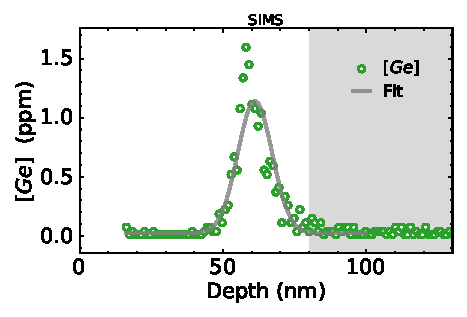
\includegraphics[width=\textwidth]{pdf_temp.pdf}%{\PathToOutput/pdf_temp.pdf}
  \caption{Your caption here}
  \label{fig:your_label}
\end{figure}




\section{Replicating Table2}
\autoref{tab:t2} describes how many options are found, go missing, or expire in the dataset. An option is found if it reappears the next trading day. An option is missing for if it does not reappear the next trading day. Multiple days missing, counts as multiple options missing. Lastly, if an option is lost and expires this is noted as expired. 

We would like to note an interesting aspect of this dataset. Over 80\% of the options expire on a Saturday or a non-trading day. To handle this, we push the expiration day to the nearest Friday, presumably the nearest trading day. However, there are quite a few edge cases which would explain the discrepancy between our analysis and \citet{constantinides2013}. Further investigation is required. 

%To implement this table we use pandas market calendars to produce an array of NYSE trading days. We then assign an integer to each day and merge this to our dataframe. To determine the time an option is lost, we use a relative distance argument and take differences using the integers. This is much faster than subtracting datetime objects with conditionals on if we're getting a trading day. 




\newpage 

\thispagestyle{empty}
\begin{landscape}

\begin{table}
    \centering
   \captionsetup{font={Large}}
    \caption{ Table  2 Sample}
    
\resizebox{1.4\textwidth}{!}{
\hspace*{-4cm}
  

		\begin{tabular}{*{2}{l} *{15}{r} }
		       
		        
		         \multicolumn{2}{c}{}  & \multicolumn{7}{c}{Calls}  &  \multicolumn{1}{c}{} & 
		         \multicolumn{7}{c}{Puts} \\
		         
		          
		         \cline{3-9}
		         \cline{11-17}
		       
		         
		          \multicolumn{1}{l}{Observations} &  \multicolumn{1}{l}{} &
		          \multicolumn{3}{c}{1996-01 to 2012-01} & 
		          \multicolumn{1}{c}{} &
			\multicolumn{3}{c}{2012-02 to 2019-12} & 
			\multicolumn{1}{c}{} &
		          \multicolumn{3}{c}{1996-01 to 2012-01} & 
		          \multicolumn{1}{c}{} &
			\multicolumn{3}{c}{2012-02 to 2019-12} \\
		        

		       \hline
		       
		       \multicolumn{17}{c}{All trading days} \\ 
		       
		       \hline 

	
		Found &   & 
		586,454 &  & 96\% & 
		 & 
		 3,068,050 &  &95\% & 
		 & 
		 611,764 &  & 96\% & 
		 & 
		 3,210,830& &95\% 
		 \\

		
		Missing &   & 
		0 &  & 0\% & 
		 & 
		 0 &  &0\% & 
		 & 
		 0 &  & 0\% & 
		 & 
		 0& &0\% 
		 \\

		
		Expired &   & 
		25,677 &  & 4\% & 
		 & 
		 161,127 &  &5\% & 
		 & 
		 25,185 &  & 4\% & 
		 & 
		 154,825& &5\% 
		 \\

		
        \hline
        
         \multicolumn{17}{c}{Last trading day of the month} \\

	
		Found &   & 
		39,064 &  & 95\% & 
		 & 
		 725,225 & 98\% & 
		 & 
		 40,737 &  & 96\% & 
		 & 
		 745,805& &98\% 
		 \\

		
		Interpolated &   & 
		1,944 &  & 5\% & 
		 & 
		 18,399 & 2\% & 
		 & 
		 1,867 &  & 4\% & 
		 & 
		 17,476& &2\% 
		 \\

		

	        \hline
	    \end{tabular}
	
  }
  \caption*{Tracking the instances options are found, missing or expired.}
\label{tab:t2}
\end{table}

\end{landscape}
\newpage



\section{Data}

Our option data is queried from OptionMetrics provided by Wharton Research Data Services (WRDS). We limit the query to SECID = 108105, S\&P 500 Index - SPX. We use the three month Tbill as our interest rate, this is from the Federal Reserve Board's H15 report supplied by WRDS. 

In comparison to their data, we have pulled 184 more options than them. It is unclear where the discrepancy lies. We assumed we were off by a day however this will truncate or elongate the dataset by over 300 points. We credit the discrepancy to OptionMetrics updating their data to be more accurate. 

The following links contain the documentation and helpful links for the WRDS database: 
\begin{itemize}
\item \href{https://wrds-www.wharton.upenn.edu/pages/support/manuals-and-overviews/optionmetrics/wrds-overview-optionmetrics/}{Option Metrics Overview} 
\item \href{https://wrds-www.wharton.upenn.edu/data-dictionary/optionm_all/opprcd2023/ }{Option Metric Keys}
\item \href{https://wrds-www.wharton.upenn.edu/pages/get-data/optionmetrics/ivy-db-us/options/option-prices/}{Option Metrics Query} 
\item \href{https://wrds-www.wharton.upenn.edu/data-dictionary/frb_all/rates_daily/}{Federal Reserve Report} 
\end{itemize}






\newpage
\bibliographystyle{jpe}
\bibliography{bibliography.bib}  % list here all the bibliographies that you need. 
% \bibliography{\PathToBibFile}
% \printbibliography

\newpage

\end{document}
